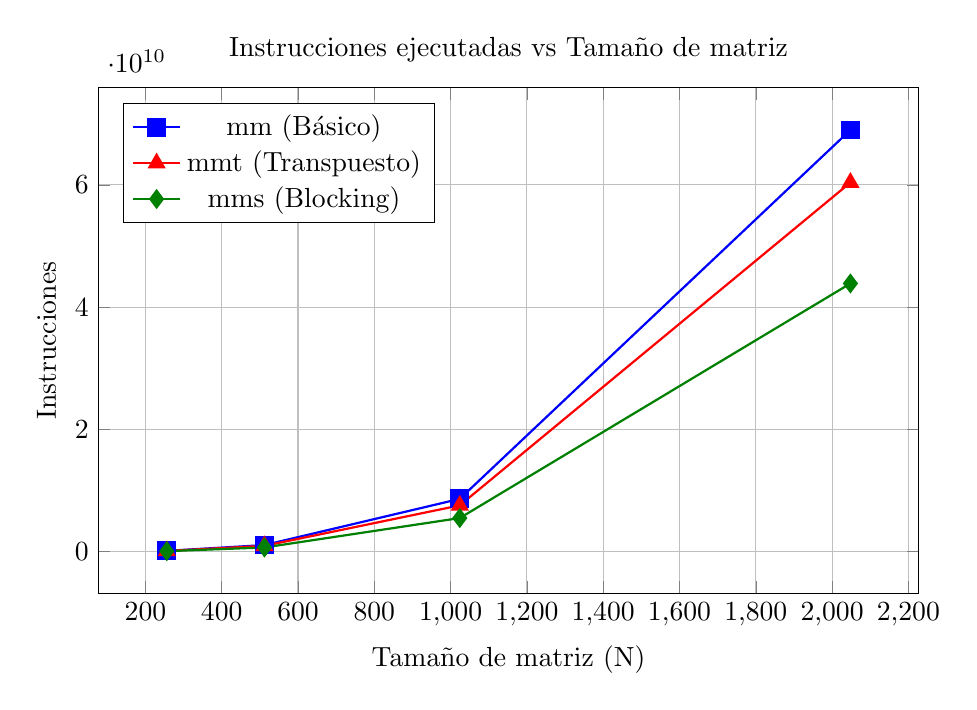
\begin{tikzpicture}
    \begin{axis}[
        title={Instrucciones ejecutadas vs Tamaño de matriz},
        xlabel={Tamaño de matriz (N)},
        ylabel={Instrucciones},
        legend pos=north west,
        grid=major,
        width=12cm,
        height=8cm,
    ]
        \addplot[
            color=blue,
            mark=square*,
            thick,
            mark size=3pt,
        ]
        coordinates {
            (256, 137758770)
            (512, 1085426559)
            (1024, 8638722142)
            (2048, 68986001315)
        };
        \addlegendentry{mm (Básico)}
        \addplot[
            color=red,
            mark=triangle*,
            thick,
            mark size=3pt,
        ]
        coordinates {
            (256, 121932710)
            (512, 954992315)
            (1024, 7576780610)
            (2048, 60392857310)
        };
        \addlegendentry{mmt (Transpuesto)}
        \addplot[
            color=green!50!black,
            mark=diamond*,
            thick,
            mark size=3pt,
        ]
        coordinates {
            (256, 88339318)
            (512, 692381169)
            (1024, 5501699730)
            (2048, 43881060286)
        };
        \addlegendentry{mms (Blocking)}
    \end{axis}
\end{tikzpicture}
